\subsection{SURF-SVM}  
SURF uses the concept of interest points (as covered in lecture 5) as a means to build a set of features that will later help establish a correspondence between two images. SURF uses windows (somewhat analogous to HOG cells), which are divided into subregions, and further subdivided into grids. By using Haar wavelets pixel intensity sums, a 4-number descriptor is obtained to define a subregion \cite{Bay2008346}.  

We used MATLAB functions \textbf{detectSURFFeatures}  to obtain SURF features and \textbf{extractFeatures} to obtain descriptors. Once again we observed that different images generated different feature numbers, so applied the same principle used to generate our HOG-SVM classifier. We used script \textbf{TrainNetworks.m} and function \textbf{fnCreateSURFSVMClassifier} to try out different parameters; results shown in Table \ref{table:surf_stats}, section \ref{Appendix}. We opted to use 50 SURF features with 200 70x70 grayscale images, as RGB images could not be used. This was not our best performing model but for the sake of having a single data for the HOG-SVM and SURF-SVM classifiers we sacrificed SURF-SVM accuracy. See section \ref{Discussion-marker} for discussion.   

To generate the matrix to fit our multiclass models for our support vector machine, we used the same approach as with our HOG-SVM, except the final vector adjustment had a slightly different implementation, to account for the 64 dimensions used in SURF.

To run our SURF-SVM classifier we used function \textbf{fnSURFSMVPredict}, again using the same principle as with the HOG-SVM classifier, where the same SURF feature number is used to make predictions, as was used to fit the classifier.  

The final SURF-SVM classifier accuracy obtained from fitting a model with 50 SURF features, 48 labels and 200 70x70 pixel grayscale images was 0.90625 (Table \ref{table:surf_stats}, section \ref{Appendix}). The confusion matrix for our best model was unreadable due to the amount of rows and columns, so we generated a second confusion matrix with 8 labels only (Figure \ref{fig:surf_conf_mat}). The accuracy obtained for the 8-label model was 96.3\%. This is assumed to be an artifact, due to individual labels presenting different classification accuracies.

\begin{figure}[h]
 \centering 
 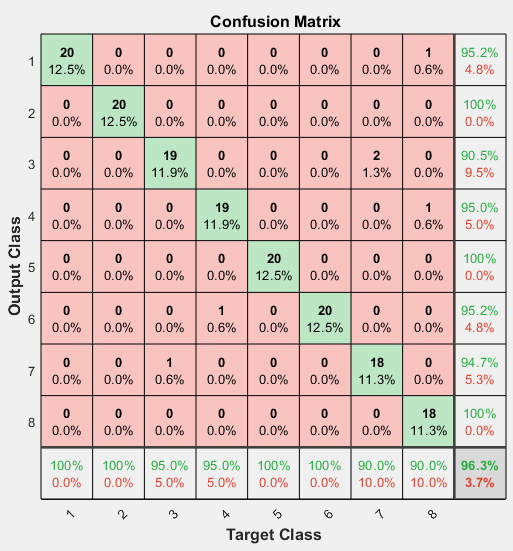
\includegraphics[width=\columnwidth]{images/SURF-SVM-Conf-Mat-200-gray-0.9.png}
 \caption{SURF SVM Confusion Matrix, 8 labels, 200 images each, 90\%/10\% train/test split}
 \label{fig:surf_conf_mat}
\end{figure} 
